%!TEX root = ../../main.tex

\chapter{Data Understanding}
\label{chap:data_understanding}

Data Profiling is the process of examining available data repeatedly throughout a project. At first light profiling assessment was undertaken. This was done using SQL and open source SQLite editors, entity relationship diagram tools and Pandas Profiling. As can be seen in the entity relationship diagram depicted in figure ~\ref{fig:erm} the data available for this project is stored in a database consisting of seven tables.
\newline
The tables "Country", "League", "Team" and "Player" hold IDs, names and foreign keys to the tables "Team\_Attributes", "Player\_Attributes" and "Match". A player's birthdate, height and weight can be found in the table "Player".
\newline
The table "Team\_Attributes" provides data on the individual teams such as playing style, defense class and so on in 12 numerical and 13 categorical columns or variables. However, 66.5 \% of the values for "buildUpPlayDribbling" are missing and therefore this variable is useless.
\newline
The table "Player\_Attributes" holds 31 numerical and 4 categorical variables and provides player statistics. Only a small percentage of values is missing.
\newline
The table "Match" holds information on football matches in Europe from 2008 until 2016 which is made up of 64 numerical and 19 categorical variables including goals scored, ball possession and odds quoted by several bookkeepers. Unfortunately a high percentage of the data on which players played in a match is missing. Moreover, ball possession and shot statistics are in XML format and not available for each match either. The odd variables (from different bookkeepers) are highly correlated.   
\newline
Together with the product owners, it was decided that this project, or at least its first phase, and the features which have to be developed will be focusing on soccer matches and their outcomes and not on individual team- or player-attributes and statistics. Therefore, the tables "Team\_Attributes" and "Player\_Attributes" are not of interest in this phase. The tables "Country", "League", "Team" and "Player" are not relevant either, since they do not hold any useful information for the first phase.


\begin{figure}[H]
\centering
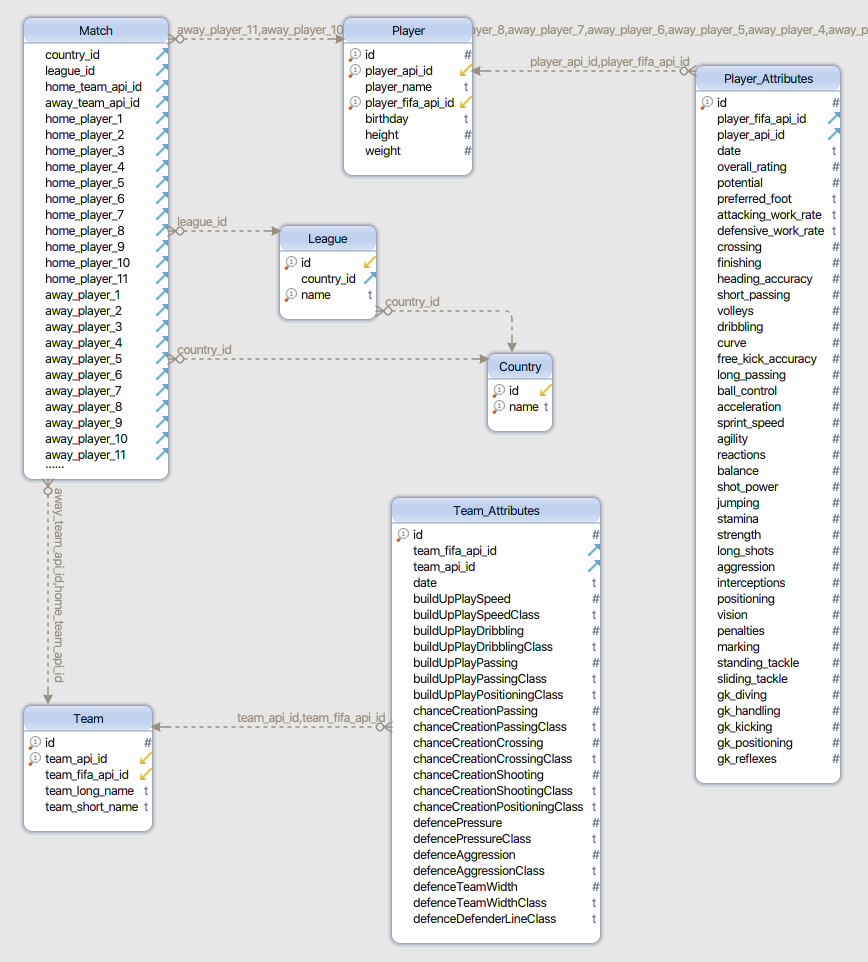
\includegraphics[width=1\textwidth]{images/erm.png}
\caption{Entity Relationship Diagram European Soccer Database}
\label{fig:erm}
\end{figure}